% !TeX root = ../../thesis.tex
\chapter{Particles with anisotropic interface energy}\label{ch_anisoIEintro}
\section{Isolated particle with anisotropic interface energy} \label{sec_isol_aniso_particle}
It was already discovered in 1901, how to determine the stable equilibrium shape of a particle with crystalline anisotropy~\cite{Wulff1901}. The chemical potential $\mu(\theta)$ must be constant along the surface of equilibrium shape~\cite{Bao2017}. Assuming that the surface is only under the influence of anisotropic capillary force, the chemical potential on the curved surface in 3D space depends on the local principal curvatures and interface energy anisotropy as follows from the Herring equation~\cite{Herring1951, Johnson1965}. In 2D the surfaces become curves and the expression for the chemical potential is simplified to
\begin{equation}\label{eq_chempot_constant}
	\mu(\theta) = \tilde{\sigma}(\theta)K \,,
\end{equation}
with local interface normal angle $\theta$ and local curvature $K$. The interface stiffness $\tilde{\sigma}(\theta)$ is the thermodynamic driving force for the capillary motion and the local curvature $\kappa$ is the thermodynamic coordinate. The interface stiffness is 
\begin{equation} \label{eq_def_interface_siffness}
	\tilde{\sigma}(\theta)=\sigma_0[h(\theta)+h''(\theta)] \,,
\end{equation}
where $h(\theta)$ and $h(\theta)''$ stand for the anisotropy function and its second derivative, respectively. The anisotropy function defines the interface energy $\sigma(\theta)$
\begin{equation} \label{eq_anisoIE}
	\sigma(\theta) = \sigma_0  h(\theta) \,,
\end{equation}
where $\sigma_0$ is a constant with physical dimensions of interface energy (i.e. $\mathrm{J/m^2}$). In this chapter it is assumed, that the anisotropy function takes the following form 
\begin{equation} \label{eq_anisofun}
	f(\theta -\alpha) = 1+\delta\cos(n(\theta-\alpha)) \,,
\end{equation}
where $0\leq\delta<1$ is the strength of anisotropy, $n$ the order of symmetry and $\alpha$ the angle rotating the anisotropy function, representing the 2D crystal orientation. A normalized strength of anisotropy $0\leq \Omega < (n^2-1)$ can be defined as $\Omega=\delta(n^2-1)$. In this paper, weak anisotropy will specifically refer to $\Omega<1$ and strong anisotropy to $\Omega\geq1$.

The interface stiffness then reads
\begin{equation}\label{eq_interface_stiffness}
	\tilde{\sigma}(\theta) = \sigma_0\{1
	-\Omega\cos[n(\theta-\alpha)]\} \,.
\end{equation}

The isolated particle with anisotropic interface energy takes on the well-known Wulff shape, which in 2D can be described as a parametric curve $\bm{w}(\theta)=[w_x(\theta),w_y(\theta)]^\mathrm{T}$\cite{Burton1951,Kobayashi2001,Eggleston2001}
\begin{align} 
	w_x(\theta) &= R_W[h(\theta)\cos(\theta) - h'(\theta)\sin(\theta)] \label{eq_wulff_parametrically_x}\\
	w_y(\theta) &= R_W[h(\theta)\sin(\theta) + h'(\theta)\cos(\theta)] \label{eq_wulff_parametrically_y}\,.
\end{align}
See Figure~\ref{fig_wulff_intro} for examples of 4-fold symmetry at various strengths of anisotropy $\delta$. 
\begin{figure}[t]
	\centering
	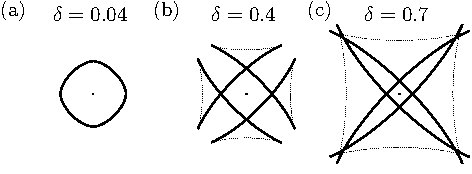
\includegraphics[page=1]{combine_graphs.pdf}
	\caption{Examples of full Wulff plots (i.e. $-\pi\leq\theta\leq\pi$) of 4-fold symmetry with indicated strengths of anisotropy. The dotted segments are the forbidden orientations, solid lines are the allowed ones. The "ears" in b) do not contribute to the isolated particle shape. However, at even stronger anisotropy in c) another intersection occurs among the branches, which introduces new solutions to the equilibrium shape.}
	\label{fig_wulff_intro}
\end{figure}

From equation~\eqref{eq_interface_stiffness}, it is easily seen that for $\Omega>1$, there are such $\theta$s, for which the interface stiffness is negative. These normal angles are unstable~\cite{Eggleston2001, Kobayashi2001,Bao2017}, hence they do not occur on the stable equilibrium Wulff shape (see the dotted segments in Figure~\ref{fig_wulff_intro}) and are called missing or forbidden. Closer inspection of the anisotropy function~\eqref{eq_anisofun} and its derivatives reveals that the forbidden angles correspond to interface energies near maxima of the anisotropy function. In fact, the latter is a general observation, independent on the particular anisotropy function~\eqref{eq_anisofun}.

For $\Omega>1$, the equations~\eqref{eq_wulff_parametrically_x}-\eqref{eq_wulff_parametrically_y} must be understood in a piece-wise fashion for the intervals of allowed $\theta$s. Each of these allowed-angles interval produces a single branch in the Wulff curve. The discontinuity in allowed angles causes that the Wulff shape is no longer a smooth and continuous closed curve (like in Figure~\ref{fig_wulff_intro}a). Instead, it is a piece-wise continuous and self-intersecting curve (Figure~\ref{fig_wulff_intro}b-c), where the individual branches enclose a polygon-like closed curve with corners. In the case of Figure~\ref{fig_wulff_intro}b, the outer parts of the shape (so-called ears) cannot contribute to the (isolated) crystal shape, but for strong enough anisotropy (like in Figure~\ref{fig_wulff_intro}c) the ears cross again, giving rise to a multitude of other stable equilibrium solutions. That is because every single of the four spikes can be part of the solution but does not need to be. This repeated crossing of the ears and its implications for the equilibrium shapes have not been reported in any work known to the author, hence it will be elaborated on in detail. 

\begin{figure*}[h]
	\centering
	\includegraphics[width=\textwidth, page=2]{combine_graphs.pdf}
	\caption{Orders of corners, defined by the branches intersections, shown for 6-fold anisotropy and $\delta=0.7$. In a) there are all the allowed angles, in b)-d) are the stable equilibrium shapes defined by the b) first order, c) second order and d) third order of the corners. Any closed curve is a stable equilibrium shape, which connects these corners along the allowed-angles branches and has the interface normals pointing outwards in every point.}
	\label{fig_wulff_cross_orders}
\end{figure*}

To emphasize the general features of this "crossed-ears" type of solutions, the Figure~\ref{fig_wulff_cross_orders}a provides another example of very strong, but 6-fold anisotropy, where the ears cross even twice behind the polygon-like isolated Wulff shape. Then, Figures~\ref{fig_wulff_cross_orders}b-d show the different possible shapes, where the outer corners always correspond to branch intersection of the same type. The type of intersection can be characterized by the radial distance from the center, based on which they can be ordered. Practically, the corner of the first order is a corner on the polygon-like shape, where two branches forming adjacent sides of the polygon-like shape cross (Figure~\ref{fig_wulff_cross_orders}b). A corner of the second order is farther from the center and is the intersection of two branches forming two polygon sides separated by a single side (Figure~\ref{fig_wulff_cross_orders}c). A corner of the third order (Figure~\ref{fig_wulff_cross_orders}d) is the intersection of two branches separated by two sides etc.

\begin{table}[b]
	\centering
	\begin{tabular}{c|c|c|c}
		\hline
		& \multicolumn{3}{c}{order of corner}      \\ 
		$n$ & 1                 & 2                 & 3                  \\ \hline
		4   & 0.06667  & 0.60000  & x                  \\
		& (1.00000) & (9.00000) & \\
		6   & 0.02857  & 0.16422  & 0.62136  \\
		& (1.00000) & (5.74773) & (21.74773)\\
		\hline
	\end{tabular}
	\caption{The approximate minimal strengths of anisotropy at which the corners of indicated order appear on the Wulff shapes in 4-fold and 6-fold anisotropy. The first number is the strength of anisotropy $\delta$ and in parenthesis is the corresponding normalized strength of anisotropy $\Omega=\delta(n^2-1)$.}
	\label{tab_soa_ears_crossing}
\end{table}

For convenience, the shapes in Figures~\ref{fig_wulff_cross_orders}b-d will be called isolated Wulff shapes of first, second and third order, respectively.

Below, a summary of some key points is given:
\begin{itemize}
	\item for $n\geq2$ and $\delta\geq 1/(n^2-1)$ the Wulff shape comprises of $n$ mutually crossing branches and the isolated shape (of first order) exhibits corners,
	\item for $n\geq4$ multiple branches intersections occur for sufficiently large $\delta$,
	\item the branches intersections (corners) can be characterized by their radial distance from the center,
	\item the upper limit on the number of intersections of a single branch with others depends on the total number of branches, i.e. on the order of symmetry $n$,
	\item as long as the orientation of the curve is respected (i.e. interface normal of all segments on the shape points outwards), any closed curve connecting the above mentioned corners along the branches is a stable equilibrium shape,
	\item the shape of higher order contains all the lower-order shapes and has larger area than any of them. The first-order shape thus has the smallest area and, consequently the least total interface energy. 
\end{itemize}

In Table~\ref{tab_soa_ears_crossing}, there are provided the minimal strengths of anisotropy at which the corners of indicated order appear on the Wulff shape in 4-fold and 6-fold anisotropy. Of these, only the first-order corners have an analytic expression, the higher-order corners were obtained numerically and thus are only approximate.

\section{Particle with anisotropic interface energy on a plane (Winterbottom construction)}
\begin{figure*}[h]
	\centering
	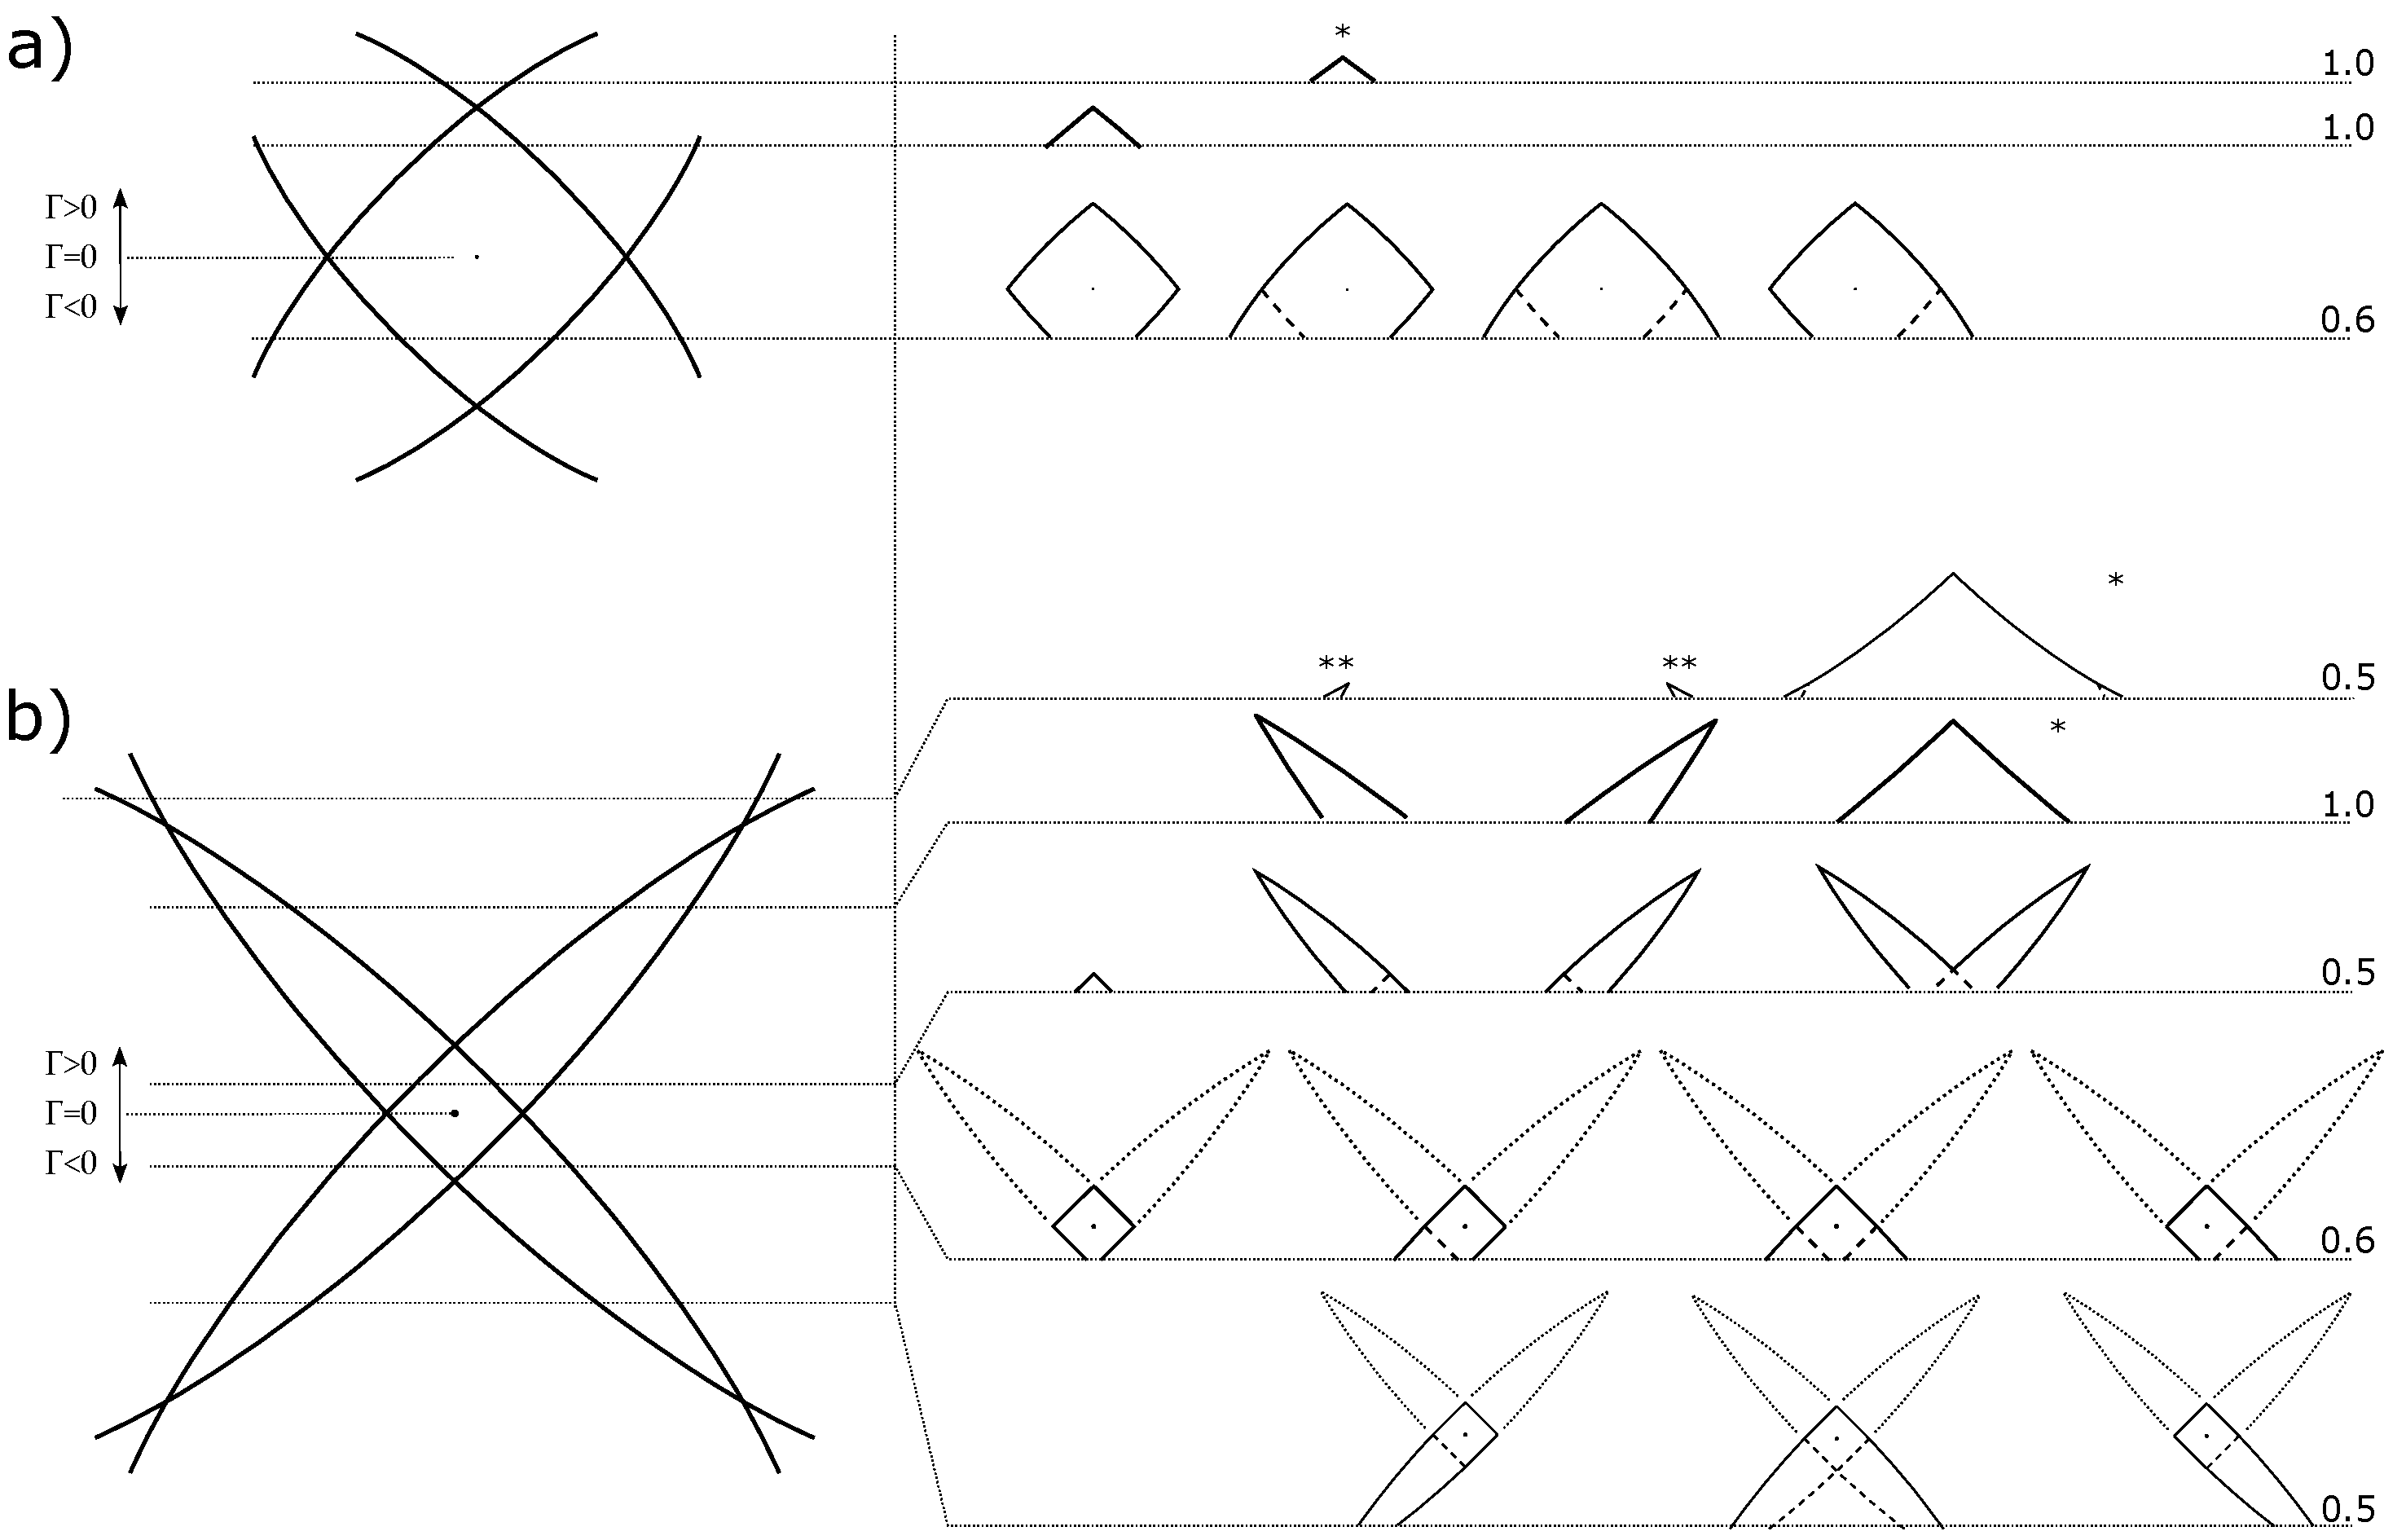
\includegraphics[width=\textwidth]{Wulff_on_plane_stronganiso.pdf}
	\caption{Complete list of non-trivial equilibrium shapes of a particle with anisotropic interface energy on a plane (right part of the sketches) as derived from full Wulff shapes (left part of the sketches) using generalized Winterbottom construction. In a) for strength of anisotropy $\delta=0.3$, in b) with $\delta=0.7$. The horizontal dotted lines indicate different truncating lines for the Wulff shape and at the same time the substrate for the equilibrium shapes. The scale of the equilibrium shapes relative to the full Wulff shapes on the left is provided on the right on every respective line. Inverted shape solutions of first order are indicated by asterisk *, of the second order by **. The dashed lines within some of the the equilibrium shapes show the segments on the Wulff shape which were enclosed by the equilibrium shape. The dotted lines above the equilibrium shapes in b) indicate the crossed-ears solutions, which either may be present both, separately or both be absent. The new solutions can be seen in b).}
	\label{fig_wulffonplane_solutions_sketches}
\end{figure*}
The problem of equilibrium shape of a particle with anisotropic interface energy on a planar substrate was treated in various works. It can either be derived from variational principles by total interface energy minimization~\cite{Winterbottom1967, Mariaux2011} or by the Cahn-Hoffman vector formalism~\cite{Cahn1974}. 

The shape is strongly determined by the force balance of the three meeting interfaces: substrate-parent phase ($\sigma_1$), particle-parent phase ($\sigma_2$) and particle-substrate ($\sigma_3$). There are two such contact points in 2D (in 3D it is a triple line) and both must be in force balance in order to sustain a stable equilibrium shape. 

Winterbottom construction identifies which segments on the full Wulff shape are (or can be) part of the equilibrium shape of a particle with anisotropic interface energy on a plane. 

For tractability of the general solution (of the particle shape), it is essential to assume co-planarity of the particle-substrate and substrate-parent phase interfaces~\cite{Winterbottom1967, Cahn1974, Bao2017}. 

In 2D, the stability of the shape derives from the stability of the two contact points. In this geometry, all interface energies are known and the orientations of two of the interfaces are known (the former substrate plane). The orientation of the last interface (the particle) in the left and right contact points are expressed by normal angles $\theta_c^L,\theta_c^R$, respectively. These are found using the Young's equation with inclination dependence, solved in every contact point 
\begin{equation}\label{eq_Young_anisotropic}
	\sigma_1 - \sigma_{3} = \sigma_2(\theta_2)\sin(\theta_2) + \sigma_2'(\theta_2)\cos(\theta_2) \,,
\end{equation}
which can be written in a non-dimensional form
\begin{equation} \label{eq_nondim_aniso_young}
	\Gamma = h(\theta_2)\sin(\theta_2) + h'(\theta_2)\cos(\theta_2) \,,
\end{equation}
where $\Gamma = [\sigma_{1}-\sigma_3 ]/\sigma_2^0$ will be denoted \textit{wetting parameter} in this paper. It can be both positive or negative. 

The solutions are from the ranges $3\pi/2>\theta_c^L>\pi/2$ and $\pi/2>\theta_c^R\geq-\pi/2$ and must be allowed angles. When~\eqref{eq_nondim_aniso_young} is compared to~\eqref{eq_wulff_parametrically_y}, it is obvious that the solutions $\theta_c^L,\theta_c^R$ are found as normal angles in points with y coordinate equal to $\Gamma$ on an unit-radius Wulff shape.  Thus, the resulting particle shape is a segment of the isolated shape, where the position of the sectioning plane $\Gamma$ is determined by the force balance. That is the Winterbottom construction. Originally, it served to find the shape of the least interface energy, but Bao~\cite{Bao2017} generalized it for any stable equilibrium shape. For illustration of the generalized Winterbottom construction depending on the position of the truncating line see Figure~\ref{fig_wulffonplane_solutions_sketches}.

When the anisotropy is strong, multiple stable equilibrium shapes may exist even when the isolated shape has only a single equilibrium stable shape. All these solutions are illustrated in Figure~\ref{fig_wulffonplane_solutions_sketches}a for 4-fold anisotropy, moderately strong~\cite{Bao2017}. In  Figure~\ref{fig_wulffonplane_solutions_sketches}b all possible solutions are presented for very strong 4-fold anisotropy, which involves the new solutions derived from the second-order corners.

If multiple solutions existed in the isolated particle in the above-truncating-line part, this multiplicity is present in the possible solutions on the plane too (Figure~\ref{fig_wulffonplane_solutions_sketches}b). Compared to the isolated case, additional solutions are present, when the truncating line passes below the center of the isolated shape, with the shape being defined also by the "ears" extending behind the corners (in both Figure~\ref{fig_wulffonplane_solutions_sketches}a and~\ref{fig_wulffonplane_solutions_sketches}b).

An exceptional class of the solutions is the \textit{inverted shape solution} (indicated by asterisk in Figure~\ref{fig_wulffonplane_solutions_sketches}), which is found \textit{below} the sectioning plane, as described by Bao~\cite{Bao2017} on a shape like in Figure~\ref{fig_wulffonplane_solutions_sketches}a. However, due to the inverted shape symmetry, it is not clear, what operation(s) of symmetry the "inversion" refers to according to Bao and how to construct the solution in a general case. More detailed characterization of this solution type was given in the following section \ref{sec_inverted_Winterbottom}. It should be noted that in systems with corners of higher order, multiple orders of the inversion shape are possible (also indicated in Figure~\ref{fig_wulffonplane_solutions_sketches} by asterisk * and described in more detail in~\ref{sec_inverted_Winterbottom}).

\section{Inverted solution in Winterbottom construction} \label{sec_inverted_Winterbottom}
The inverted shape in a Winterbottom construction with single plane was described by~\cite{Bao2017} in a highly symmetric case. The same idea was used much sooner in the Winterbottom construction in a corner (meaning Wulff shape resting on two lines at once, intersecting in a corner) by Zia et al.~\cite{Zia1988} ("Summertop construction"). Below, the inverted shape construction is described, taking into account the higher-order intersection solutions and arbitrary rotations.

Let the Wulff shape exhibit strong anisotropy, i.e. be there at least corners of first order. Further, let the wetting parameter $\Gamma$ be such, that the truncating line passes at least above the isolated shape of the first order, i.e. the first-order shape is submerged below the substrate plane. 
\begin{figure}[]
	\centering
	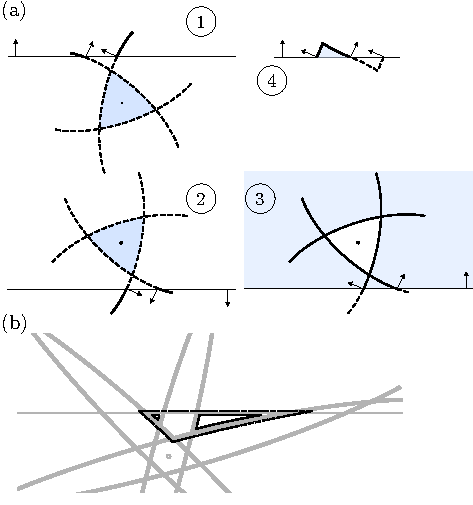
\includegraphics[width=0.6\textwidth]{fig_inverted_sol.pdf}
	\caption{Illustration of the inverted Winterbottom construction. In (a) explained in 4 steps and in (b) illustration of inverted solutions of higher orders. In (a) the plane normal points from the substrate to the parent phase, the solid lines of the Wulff plot are thus above the substrate plane and the dashed ones are below. Interface normals in the contact points are indicated as well. In 1 is the initial state, in 2 after center inversion, in 3 after the curve orientation flip and in 4 is the resulting shape next to the original part of the Wulff plot. In (b) the dashed black line indicates inverted shape of the first order, the solid line that of second order.}
	\label{fig_inverted_explained}
\end{figure}

Then it may happen, that the truncating line intersects two branches, which crossed below it (see Figure~\ref{fig_inverted_explained}a1). Such situation allows a solution, where the equilibrium shape is the part \textit{below} the substrate plane, but \textit{above} the corner where the two branches intersect. Two steps must be followed to obtain the inverted equilibrium shape:
\begin{enumerate}
	\item point inversion of the whole system (Wulff plot + truncating line) about the center of the Wulff shape (see Figure~\ref{fig_inverted_explained}a2)
	\item flip orientation of both the inverted Wulff plot and inverted truncating line, i.e. flip the inverted inward and outwards  directions (see Figure~\ref{fig_inverted_explained}a3)
\end{enumerate}


The first operation places the truncating line below the said corner, where the two branches intersect. At the same time, the whole shape is inverted. The second operation turns the outside of the Wulff plot to be inside - i.e. instead of having a a crystal in the shape of inverted Wulff plot in some medium, we have a medium in the shape of Wulff plot surrounded by the crystal. 

Then, the resulting inverted shape as in Figure~\ref{fig_inverted_explained}a4 is obtained as an enclosed intersection of the anisotropic Wulff plot and a half-space above the line. All the interface normal orientations on the surface of the inverted shape are the same as on the non-inverted part of the Wulff plot. Importantly, this includes the normal angles in the contact points, as can be seen in Figure~\ref{fig_inverted_explained}a4.

The order of the intersection in which the two Wulff branches intersect, determines the order of the inverted shape. Figure~\ref{fig_inverted_explained}b shows an example of strong 6-fold anisotropy with such truncation, that it allows two orders of inverted shapes at once.


\section{Contact point stability}
The contact points mentioned above are essentially triple junctions. The Young's equation with inclination dependence~\eqref{eq_Young_anisotropic} represents equilibrium of the tractions due to the interfaces on the junction in the $x$ direction. It concerns
a special case, where the position of two of the three interfaces are fixed to lay on the x axis and the third has inclination-dependent interface energy. However, the \textit{stability} of the triple junction configuration is not guranteed by Young's equation alone~\cite{Marks2012}. In the present case, the configuration means a solution $\theta_2$ to~\eqref{eq_Young_anisotropic}. Technically, the solutions to~\eqref{eq_Young_anisotropic} are stationary points of the triple junction energy as function of virtual translations, but not necessarily its minimum (i.e. the stable configuration). Stability of the found solutions should be thus tested using additional conditions derived from second-order derivatives of the triple junction energy with respect to the virtual translations~\cite{Marks2012}:
\begin{align} 
	0 &< \tilde{\sigma}_1 s_1 + \tilde{\sigma}_2 s_2 + \tilde{\sigma}_3 s_3 \\
	0 &< \tilde{\sigma}_1\tilde{\sigma}_2 S_{12} + \tilde{\sigma}_2\tilde{\sigma}_3 S_{23} + \tilde{\sigma}_1\tilde{\sigma}_3 S_{13} \,,
\end{align}
where $\tilde{\sigma}_i$ are the respective interface stiffnesses, $s_i = \cos^2(\theta_i)/d_i$, $S_{ij} = \sin^2(\theta_i-\theta_j)/d_i d_j$. In the present geometry, interfaces 1 and 3 are fixed with $\theta_1=\pm\pi/2$ and $\theta_3=\mp\pi/2$, hence it follows that $s_1=s_3=0$ and also that $S_{13}=0$. Note also that $s_2>0$ and $S_{12}=S_{23}=S>0$. By the geometry alone, the conditions are thus simplified to
\begin{align}
	0 &< \tilde{\sigma}_2  \label{eq_3jun_stabcond_onplane1}\\
	0 &< \tilde{\sigma}_1\tilde{\sigma}_2 + \tilde{\sigma}_2\tilde{\sigma}_3 \,,  
\end{align}
where only the interface stiffnesses matter. Using the first equation, the second one may further be simplified
\begin{equation}
	0< \tilde{\sigma}_1 + \tilde{\sigma}_3 \,. \label{eq_3jun_stabcond_onplane2}
\end{equation}
The condition~\eqref{eq_3jun_stabcond_onplane1} implies, that the particle-parent phase interface must be oriented under allowed angle in the contact point. That is fulfilled automatically by the truncated Wulff shape solution, because it contains only the allowed angles. 

Note that the interfaces 1 and 3 have fixed orientations and are assumed to be planar. The condition~\eqref{eq_3jun_stabcond_onplane2} is surely fulfilled when both interfaces 1 and 3 have positive interface stiffness in their orientations. That holds automatically in weak or no anisotropies. When either or both of the two interfaces exhibit strong anisotropy, it means that there are normal angles where the interface stiffness is negative, hence the condition~\eqref{eq_3jun_stabcond_onplane2} may be violated and must be verified in the given configuration.

\section{Selected geometric properties of Wulff shape}\label{sec_appendix_anisofun_props}
With $h(\theta)=1+\delta\cos(n\theta)$, the minimal distance $R_{min}$ between the Wulff shape center and the contour can be related to $R_W$ as
\begin{equation} \label{eq_appdx_wulff_minradius}
	R_{min} = R_W(1-\delta) \,,
\end{equation}
which holds for arbitrarily strong anisotropy because the minimal-radius point normal is always inclined under a non-missing angle. This formula was used to find the radius $R_W$ of the phase field contour. Then, the phase field contour was scaled to unit radius and compared to the analytic Wulff shape (by means of Hausdorff distance, see the next subsection). 

The radius of curvature $\varrho(\theta)$ of Wulff shape is locally
\begin{equation} \label{eq_Wulff_radius_curvature}
	\varrho(\theta) = R_W[h''(\theta) + h(\theta)] \,,
\end{equation}
which may technically get negative for some $\theta$. Because that does not have any geometric interpretation, the Wulff shape does not contain such oriented segments and the angles $\theta_m$ fulfilling $\varrho(\theta_m)\leq0$ are called missing or forbidden. \\

For a given radius $R_W$, the area of a Wulff shape $A_W$ differs from the area of a circle $A=\pi R_W^2$ by the anisotropy-dependent factor $C_W(\Omega,n) = A_W/A$. For weak anisotropy $\Omega<1$ there is an analytic expression 
\begin{equation}
	C_W = 1-\frac{\Omega^2}{n^2-1} \,,
\end{equation}
but there is none for strong anisotropy $\Omega>1$. The factor $C_W(\Omega,n)$ was obtained numerically for $n=4$ in the range $0\leq\Omega\leq7.5$ (the Wulff shape was plotted, its area numerically computed and divided by $\pi R^2$). There, the $\Omega$-dependence was fitted very well  by a polynomial of 4-th order $C_W(\Omega,4)= \sum_{i=0}^4a_i\Omega^{N-i}$ with $a_0=-0.00032 ,a_1=0.00639 ,a_2=-0.04219 , a_3=0.00034 , a_4=1.00000$. 

\section{Shrinkage rate of a Wulff shape} \label{sec_appendix_wulff_shrrate}
The normal velocity of anisotropic curvature-driven interface in 2D is~\cite{Abdeljawad2018}
\begin{equation}
	v_n(\theta,t)=-\frac{\mu}{\varrho(\theta,t)}\sigma_0[h''(\theta) + h(\theta)] 
\end{equation}
where $\mu$ is the interface mobility and $\sigma_0[h''(\theta) + h(\theta)]$ is interface stiffness. When it is the
Wulff shape shrinking, the radius of curvature $\varrho(\theta,t)$ can be expressed as in equation~\eqref{eq_Wulff_radius_curvature} and the inclination-dependent part of the interface stiffness is cancelled out. The normal velocity is then constant along the perimeter
\begin{equation} \label{eq_wulff_norm_velocity}
	v_n(t) = - \frac{\mu \sigma_0}{R_W(t)} \,.
\end{equation}
The sign is such that the interface moves towards the center of curvature.

Because the area of a Wulff shape is $A_W=\pi R_W^2C_W(\Omega,n)$, the shrinkage rate of a Wulff shape is
\begin{equation}\label{eq_wulff_shrrate_deriv}
	\begin{split}
		\frac{\mathrm{d}A_W}{\mathrm{d}t} &= \frac{\mathrm{d}}{\mathrm{d}t}[\pi R_W^2(t)C_W(\Omega,n)]    \\
		&= 2\pi C_W(\Omega,n) R_W(t) \frac{\mathrm{d}R_W}{\mathrm{d}t} \,.
	\end{split}
\end{equation}
Because  the normal velocity is constant along the perimeter, the point $R_{min}$ from equation~\eqref{eq_appdx_wulff_minradius} moves also by $v_n(t)$. Importantly, the normal of interface in $R_{min}$ is aligned with the radial direction of the polar coordinates, hence we can write $v_n=\mathrm{d}R_{min}/\mathrm{d}t$. From equation~\eqref{eq_appdx_wulff_minradius} then must be
\begin{equation}
	\frac{\mathrm{d}R_{W}}{\mathrm{d}t}=\frac{1}{1-\delta}\frac{\mathrm{d}R_{min}}{\mathrm{d}t}=\frac{1}{1-\delta}v_n(t) \,,
\end{equation}
which together with~\ref{eq_wulff_norm_velocity} implies in \ref{eq_wulff_shrrate_deriv}
\begin{equation}
	\frac{\mathrm{d}A_W}{\mathrm{d}t} = 2\pi\mu\sigma_0  \frac{C_W(\Omega,n)}{1-\delta} 
\end{equation}

Taylor and Cahn~\cite{Taylor1998} proved that the shrinkage rate for the equilibrium shape must be a constant, which is met by the final expression.


\section{Summary and the author's contribution}
This chapter contained fundamental information about the equilibrium stable shapes of particles with anisotropic interface energy, assuming absence of other driving forces which might affect their shape. Isolated particles as well as those on a plane were assessed in 2D. New stable equilibrium shapes were described in the case of very strong anisotropy, where the Wulff plot may self-intersect multiple times, thus giving rise to the solutions containing parts formed by crossed "ears". The notion of "order of the intersection" was introduced to generalize the description of the emerging solution type. 

Regarding the particle on a plane, the inverted solution type was described in detail allowing its construction for arbitrary nucleus orientation and wetting. Inverted solutions of higher orders were described as well.

The author is not aware of another work applying the stability conditions for the triple junction configuration to the nucleus contact points. Later, it is shown that for particles with strongly anisotropic interface energy, the stability condition is a very strong influence on the orientation selection in repeated nucleation.

Some basic geometric properties of the Wulff shapes were reviewed, which were later utilized in the phase-field model benchmarkig. Specifically, the steady-state shrinkage rate of a Wulff shape is an useful formula derived by the author.


%\section{Capillary vector formalism}
%Let the interface energy $\sigma$ depend on the local orientation of the interface described by its unit normal $\bm{n}$, i.e. $\sigma=\sigma(\bm{n})=\sigma_0 f(\bm{n})$. The function $f(\bm{n})$ is called anisotropy function and $\sigma_0$  is a scaling parameter with dimensions of interface energy. Formal requirements on the anisotropy function can be found e.g. in~\cite{Kobayashi2001}. A very useful formalism for thermodynamic description of these anisotropic interfaces is so-called capillary vector $\bm{\xi}$ (a.k.a. Cahn-Hoffmann vector or $\xi$-vector), defined as 
%\begin{equation}
%     \bm{\xi} = \mathrm{grad}(r\sigma(\bm{n}))\,,
% \end{equation}
%where $r$ is radial distance from origin, which can be also seen as magnitude of scaled normal vector $\bm{r}=r\bm{n}$. Level sets of the scalar function $r\sigma(\bm{n})$ are geometrically similar to the anisotropy function $f(\bm{n})$, which is continuously scaled by the radius $r$.
%
%Capillary vector was introduced and investigated by Hoffman and Cahn in~\cite{Hoffman1972,Cahn1974}, who showed that this formalism is consistent with major laws governing behavior of (anisotropic) interfaces like Gibbs-Thompson equation (relating chemical potential and isotropic surface curvature), Herring's equation (chemical potential on anisotropic curved surface), Wulff shape construction, force balance at multi-junctions and others. 
%
%A defining property of capillary vector is that its component normal to the surface $\xi_\perp$ is in magnitude equal to the local value of the interface energy and the surface-tangent component points in the direction of steepest change in interface energy and is proportional to the change. More specifically  
%\begin{align}
%     \xi_\perp &= \bm{\xi}\cdot\bm{n}=\sigma(\bm{n}) \\
%     \xi_\| &= \left(\frac{\partial \sigma}{\partial \theta}\right)_{max} \,,
% \end{align}
%where $\theta$ is the angle representing change in orientation of $\bm{n}$ in the direction of maximal angular rate change. The vector can thus be written
%\begin{equation}
%     \bm{\xi}(\bm{n}) = \sigma(\bm{n})\bm{n} + \left(\frac{\partial \sigma}{\partial \theta}\right)_{max} \bm{t} \,,
% \end{equation}
%with $\bm{t}$ being unit vector tangent to the surface pointing in the described direction. Useful is expression of capillary vector in spherical coordinates 
%\begin{equation}
%     \bm{\xi}(\theta,\phi) = \sigma(\theta,\phi)\bm{\hat{r}} + \left(\frac{\partial \sigma}{\partial \theta}\right)\bm{\hat{\theta}} + \frac{1}{\sin(\theta)}\left(\frac{\partial \sigma}{\partial \phi}\right)\bm{\hat{\phi}} \,,
% \end{equation}
%which is only function of the polar and azimuthal angle $\theta,\phi$, respectively. In 2D in polar coordinates the normal and tangent vector can be written as functions of the interface normal angle $\theta$ as
%\begin{equation} \label{eq_xivec_2D}
%     \bm{\xi}(\theta) = \sigma(\theta)\begin{bmatrix}
%           \cos(\theta)  \\
%           \sin(\theta) 
%      \end{bmatrix} + \left(\frac{\partial \sigma}{\partial \theta}\right)\begin{bmatrix}
%           -\sin(\theta) \\
%           \cos(\theta)  
%      \end{bmatrix} \,.
% \end{equation}
%
%\section{Interface stiffness}
%
%\section{Wulff shape}
%Wulff shape is such shape, which minimizes the interface energy given a constant volume. In 2D it can be obtained as the inner convex hull of all tangent straight lines to the anisotropy function $h(\theta)$. This can be used to define the Wulff shape $W$ as a set of points $\bm{x}$
%\begin{equation}
%     W = \{ \bm{x}\in\mathbb{R}| \bm{x}\cdot\bm{n}\leq \sigma(\bm{n})\} \,,
% \end{equation}
%which is a geometrical representation of what was said above - projection of the position vector $\bm{x}$ of a point within the Wulff shape to the interface normal vector $\bm{n}$ must be smaller than the anisotropic interface energy. This defines the inner hull of the tangent lines.
%
%When the heads of capillary vectors for all interface normal angles $\theta$ are connected (having a common starting point in the origin), so-called $\xi$-plot is obtained. It turns out, that the $\xi$-plot coincides with the Wulff shape~\cite{Hoffman1972}. Hence, the expression~\eqref{eq_xivec_2D} can be used to plot the 2D Wulff shape in cartesian coordinates. This is entirely true as long as there are no corners or facets on the Wulff shape, in which cases the use of capillary vecor for Wulff shape plotting must be appropriately modified (see below for details).
%
%In~\cite{Cahn1974} the authors re-state he problem of finding equilibrium shapes of crystals with anisotropic interfaces under general conditions. The shape is found as a solution to equation
%\begin{equation} \label{eq_xivec_equilibrium_shape}
%     \Delta\Omega_v + \nabla_S\cdot \bm{\xi} = 0 \,,
% \end{equation}
%where $\Delta\Omega_v$ is the bulk driving force, specifically the difference in grand-canonical potential of the two phases, and $\nabla_S\cdot$ is surface divergence. The surface $\bm{r}$ is seeked, complying with the above equation. A simple trick is used to find the shape of an isolated particle. Surface divergence over the surface itself is simply $\nabla_S\cdot\bm{r}=2$, hence we can write
%\begin{align}
%     1 = \nabla_S\cdot\bm{r}/2 &= -\nabla_S\cdot\bm{\xi}/\Delta\Omega_v \\
%      \nabla_S\cdot(\bm{r} +2\bm{\xi}/\Delta\Omega_v) &=0 \,,
% \end{align}
%leading to the result
%\begin{equation}
%     \bm{r} = -\frac{2}{\Delta\Omega_v}\bm{\xi} \,.
% \end{equation}
%
%Two different types of singularities may occur in Wulff shapes, which must be treated in a specific way: corners and facets. 
%
%Corners represent a discontinuity of normal angle along the Wulff shape perimeter. They occur when the anisotropy of the interface energy is such, that interface stiffness gets negative for some normal angles $\theta_f$. These angles are called forbidden and they are thermodynamically unstable. For this reason, they are not present on the Wulff shape. Additionally, there are normal angles $\theta$ which are thermmodynamically stable but are not present on the Wulff shape. The latter ones correspond to angles, where the inverse interface energy $1/\sigma(\theta)$ is non-convex but still have positive interface stiffness. All forbidden angles fall into this non-convex region. By replacing the non-convex part of this function by straight lines a regularized inverse anisotropy function $1/\bar{\sigma}(\theta)$ is obtained. Wulff shape corresponding to the regularized anisotropy function $\bar{\sigma}(\theta)$ does not contain the "ears" behind the corners. The interface stiffness of both the allowed and forbidden angles which form the "ears" were thus set to zero.
%
%The facets were not treated in this work, hence they are not further discussed.
%
%\section{Force balance in triple junction and stability of its configuration} \label{sec_intro_trijun_forcebalance_stability}
%A triple junction in 2D is simply a point and force balance is achieved if the capillary vectors of the three interfaces sum to zero, i.e. 
%\begin{equation} \label{eq_trijun_forcebalance_sum_xivec}
%     \bm{\xi}_{12}+\bm{\xi}_{23}+\bm{\xi}_{13}=0
% \end{equation}
%The problem of force balance in triple junctions was treated in detail in~\cite{Marks2012}. Even though the capillary vector formalism was not used, a condition equivalent to~\eqref{eq_trijun_forcebalance_sum_xivec} was obtained from geometrical arguments (note that the 90-degree rotation does not change meaning of the equation)
%\begin{equation} \label{eq_force_balance_3jun_aniso}
%     \sum_{i=1}^3 \left[ \sigma_i(\vartheta_i)\hat{\bm{t}}_i +\frac{\mathrm{d} \sigma_i}{\mathrm{d} \vartheta_i}\hat{\bm{n}}_i \right] = 0 \,,
% \end{equation}
%where the subscripts now denote interfaces numbered from 1 to 3. $\vartheta_1,\vartheta_2,\vartheta_3$ are angles under which the tangent of each interface is oriented (all w.r.t.\ x axis),  the anisotorpic interface energies are $\sigma_i(\vartheta_i)$. The triple junction configuration is defined by the triplet of the angles $\vartheta_i$. However, it was pointed out, that the above condition is only necessary for the triple junction configuration to be stable, i.e. it does not guarantee the configuration stability. Validity of~\eqref{eq_force_balance_3jun_aniso} assures a stationary point in Gibbs free energy, but in order to have a stable configuration, the energy must be in local minimum. To confirm that, second derivatives of Gibbs free energy with respect to angles $\vartheta_1,\vartheta_2,\vartheta_3$ must be assessed, giving rise to the following two conditions (both of which must hold in stable configuration)
%\begin{align} \label{eq_3jun_aniso_stabcond1}
%     0 <& \sum_{i=1}^3 \left[ \frac{\mathrm{d}^2 \sigma_i}{\mathrm{d} \vartheta_i^2} + \sigma_i(\vartheta_i) \right]\frac{\sin^2(\vartheta_i)}{d_i} \\  \label{eq_3jun_aniso_stabcond2}
%     0 <& \left[ \frac{\mathrm{d}^2 \sigma_1}{\mathrm{d} \vartheta_1^2} + \sigma_1(\vartheta_1) \right]\left[ \frac{\mathrm{d}^2 \sigma_2}{\mathrm{d} \vartheta_2^2} + \sigma_2(\vartheta_2) \right] \frac{\sin^2(\vartheta_1-\vartheta_2)}{d_1d_2} +    \\
%      &\quad +\left[ \frac{\mathrm{d}^2 \sigma_2}{\mathrm{d} \vartheta_2^2} + \sigma_2(\vartheta_2) \right]\left[ \frac{\mathrm{d}^2 \sigma_3}{\mathrm{d} \vartheta_3^2} +  \sigma_3(\vartheta_3) \right] \frac{\sin^2(\vartheta_2-\vartheta_3)}{d_2d_3} + \nonumber \\
%      &\quad + \left[ \frac{\mathrm{d}^2 \sigma_1}{\mathrm{d} \vartheta_1^2} + \sigma_1(\vartheta_1) \right]\left[ \frac{\mathrm{d}^2 \sigma_3}{\mathrm{d} \vartheta_3^2} + \sigma_3(\vartheta_3) \right]  \frac{\sin^2(\vartheta_3-\vartheta_1)}{d_3d_1} \nonumber \,,
% \end{align}
%where $d_i$ are lengths from the triple junctions to anchor points, which are not relevant for the current work. Each term in the brackets is interface stiffness of the respective interface.
%
%If the second condition is equal to 0, these conditions are not conclusive, i.e. it is not possible to assess the nature of the stationary point (higher-order derivatives are needed then). 
%
%The assessment of stability of triple junction configuration is an important part of discussion of an equilibrium shape of anisotropic particle  on a substrate plane.
%
%\section{Equilibrium shapes of anisotorpic particle on planar substrate}
%This problem has attracted considerable attention since it is of high practical importance, especially in applications like nucleation, preparation of functional deposits for electrochemical catalysis or in solid-state dewetting. The classical solution to the problem is by Kaischew for crystalline anisotropy with faceted chape\textit{(ref 1.50 in Milchev), year 1951} and Winterbottom1967 (interface energy as continuous function). Here it is demonstrated using the capillary vector formalism. 
%
%In the following only 2D cross section is discussed. It is assumed that the particle-substrate interface (denoted here with index 1) is linear with the substrate-parent phase (index 3), but with anti-parallel normal vector. Let the substrate plane be parallel with x axis. The particle-parent phase interface is denoted by index 2. The normal vectors of the respective interfaces in the contact point are $\hat{\bm{n}}_1=(0,-1)^{\mathrm{T}}$, $\hat{\bm{n}}_3=(0,1)^{\mathrm{T}}$ and $\hat{\bm{n}}_2$ is to be found from~\eqref{eq_trijun_forcebalance_sum_xivec}. Apparently, with the interfaces 1 and 3 fixed at orientations $\theta_1=-\pi/2$ and $\theta_3=\pi/2$, the force balance can be reduced to single equation, when the particle-parent phase capillary vector $\bm{\xi}_2$ is projected to the surface normal $\hat{\bm{n}}_S=\hat{\bm{n}}_3$. But that is merely the y-component of the capillary vector. The force balance can thus be written as
%\begin{equation}\label{eq_youngs_eq_aniso}
%     \sigma_{3}(\pi/2)-\sigma_1(-\pi/2)  
%       = \sigma_2(\theta_2)\sin(\theta_2) + \sigma_2'(\theta_2)\cos(\theta_2) \,.
% \end{equation}
%
%Geometric interpretation of this equation is that the force equilibrium in the triple junction is achieved when normal angle $\theta_2$ of the particle-parent phase interface in the triple junction is that one, which has the y coordinate of the Wulff shape equal to the difference $\sigma_{3}(\pi/2)-\sigma_1(-\pi/2) $. The equilibrium shape of anisotropic particle on a substrate is thus that of an isolated particle but truncated at a position, which derives from the force balance in the triple junction. The truncated part of isolated particle counts, which is above the truncating line.
%
%When all the three interfaces are isotropic, the well known Young's equation is obtained
%\begin{align}
%     \sigma_3-\sigma_1 &= \sigma_2\sin(\theta_2) \\
%         &= \sigma_2\cos(\vartheta_2)
%     \,,
% \end{align}
%where in the second equation it was used that $\vartheta_2=\theta_2-\pi/2$.
%
%Let's assume the anisotropy of the particle-parent phase interface $\sigma_2(\theta_2)=\sigma_2^0f(\theta_2)$. Then the wetting parameter $\Gamma$ is defined
%\begin{equation}
%     \Gamma = \frac{\sigma_{3}(\pi/2)-\sigma_1(-\pi/2) }{\sigma_2^0} \,,
% \end{equation}
%which is the vertical offset of the horizontal truncating line relative to center of the equilibrium shape of unit radius. Apparently, when $\Gamma > 0$, the line is above the Wulff shape center (the shape is submerged below the line) and there is such value of $\Gamma$, when the line is merely a tangent. That corresponds to the case of complete wetting and the contact angle is 0. For isotropic interface energy that occurs for $\Gamma=1$.
%
%On the other hand, when $\Gamma < 0$, the truncating line goes below the center (the shape is emerged above the line). There is such value of $\Gamma$ corresponding to complete non-wetting (with isotropic interface energy that is $\Gamma=-1$).
%
%\section{Stability of the equilibrium shape}\label{sec_fund_anisoIE_trijun_stability}
%Previous section showed derivation of the 2D equilibrium shape of anisotropic particle on a substrate from the triple junction force balance. However, as explained in~\ref{sec_intro_trijun_forcebalance_stability}, the stability of the solution should be assessed as well. The additional conditions~\eqref{eq_3jun_aniso_stabcond1}, \eqref{eq_3jun_aniso_stabcond2} can be re-written as
%\begin{align}
%     0 &< \Sigma_1 s_1 + \Sigma_2 s_2 + \Sigma_3 s_3 \\
%     0 &< \Sigma_1\Sigma_2 S_{12} + \Sigma_2\Sigma_3 S_{23} + \Sigma_1\Sigma_3 S_{13} \,,
% \end{align}
%where $\Sigma_i = \mathrm{d}^2 \sigma_i/\mathrm{d} \vartheta_i^2 + \sigma_i(\vartheta_i)$ are the respective interface stiffnesses, $s_i = \sin^2(\vartheta_i)/d_i$, $S_{ij} = \sin^2(\vartheta_i-\vartheta_j)/d_i d_j$. Given $\vartheta_1=0$ and $\vartheta_3=\pi$, it follows that $s_1=s_3=0$ and also that $S_{13}=0$. Note also that $s_2>0$ and $S_{12}=S_{23}=S=\sin^2(\vartheta_2)/d^2>0$ (assuming that $d_1=d_2=d_3$). The conditions are thus simplified to
%\begin{align}
%     0 &< \Sigma_2  \label{eq_3jun_stabcond_onplane1}\\
%     0 &< \Sigma_1\Sigma_2 + \Sigma_2\Sigma_3 \,,  
% \end{align}
%where only the interface stiffnesses matter. Using the first equation, the second may further be simplified
%\begin{equation}
%     0< \Sigma_1 + \Sigma_3 \,. \label{eq_3jun_stabcond_onplane2}
% \end{equation}
%The condition~\eqref{eq_3jun_stabcond_onplane1} implies, that the particle-parent phase interface must be oriented under allowed angle in the contact point. That is fulfilled automatically by the truncated Wulff shape solution, because it contains only the allowed angles. 
%
%The condition~\eqref{eq_3jun_stabcond_onplane2} is surely fulfilled when both interfaces 1 and 3 have positive interface stiffness in their orientations. That holds automatically, when the Wulff shapes of the interfaces 1 and 3 do not contain any corners. When both of them do contain corners, it means that there are normal angles where the interface stiffness is negative. Apparently, in such situation, the condition~~\eqref{eq_3jun_stabcond_onplane2} may be violated.

%%%%%%%%%%%%%%%%%%%%%%%%%%%%%%%%%%%%%%%%%%%%%%%%%%
% Keep the following \cleardoublepage at the end of this file, 
% otherwise \includeonly includes empty pages.
\cleardoublepage

% vim: tw=70 nocindent expandtab foldmethod=marker foldmarker={{{}{,}{}}}
